\documentclass[12pt,letterpaper]{article}
\usepackage[utf8]{inputenc}
\usepackage[spanish]{babel}
\usepackage{amsmath}
\usepackage{amsfonts}
\usepackage{amssymb}
\usepackage{adjustbox}
\usepackage{graphicx}
\usepackage{tikz}
\usepackage{makecell}
\usetikzlibrary{arrows.meta}
\usetikzlibrary{positioning}
\usepackage[left=2cm,right=2cm,top=2cm,bottom=2cm]{geometry}
\author{
{\Large \textbf{Grupo Nº 5}}\\${ }$\\
\textbf{Integrantes:}\\
\begin{tabular}{|c|c|}
\hline 
Nombre & Registro \\ 
\hline 
Cristhian Relox Brito            & 216183243 \\ \hline
Pedro Antonio Arce Espinoza      & 217003613 \\ \hline
Ruddy Albert Olmos Tila          & 212105779 \\ \hline
Victor Hugo Mamani Copa          & 213095671 \\ \hline
Hernan Huanca Pernea             & 200660608 \\ \hline
Raul Yampara Huarachi            & 215167287 \\ \hline
Leonardo Henry Añez Vladimirovna & 217002498 \\ \hline
Roger Miguel Aguilera Masabi	  & 216155241 \\ \hline
Extid Yeferson Moreno Marquéz    & 216084415 \\ \hline
Angel Daniel Aduviri Llave       & 215150112 \\ \hline
Cristian Alexis Catari Antelo    & 215153170 \\  
\hline 
\end{tabular} 
}
\title{
{\normalsize Universidad Autónoma Gabriél René Moreno} \\
{\small Facultad de Ingeniería en Ciencias de la Computación y Telecomunicaciones}\\
{\Large \texttt{ADM100 - GRUPO: SA}}\\ {\large \textbf{Docente:} Oscar Flores} \\ \vspace{2cm}
{\Huge El Control}
\vspace{2cm}
}

%\setcounter{secnumdepth}{0} % sections are level 1

\graphicspath{ {Imagenes/} }

\begin{document}
\date{27 de Junio, 2018}
\maketitle

\newpage

\section*{Introducción}
El control ha sido definido bajo dos grandes perspectivas, una \textbf{perspectiva limitada} y una \textbf{perspectiva amplia.} Desde la \textit{perspectiva limitada}, el control se concibe como la verificación a posteriori de los resultados conseguidos en el seguimiento de los objetivos planteados y el control de gastos invertido en el proceso realizado por los niveles directivos donde la estandarización en términos cuantitativos, forma parte central de la acción de control.
\\${ }$\\
Bajo la \textit{perspectiva amplia}, el control es concebido como una actividad no sólo a nivel directivo, sino de todos los niveles y miembros de la entidad, orientando a la organización hacia el cumplimiento de los objetivos propuestos bajo mecanismos de medición cualitativos y cuantitativos. Este enfoque hace énfasis en los factores sociales y culturales presentes en el contexto institucional ya que parte del principio que es el propio comportamiento individual quien define en última instancia la eficacia de los métodos de control elegidos en la dinámica de gestión.
\\${ }$\\
Todo esto lleva a pensar que el control es un mecanismo que permite corregir desviaciones a través de indicadores cualitativos y cuantitativos dentro de un contexto social amplio, a fin de lograr el cumplimiento de los objetivos claves para el éxito organizacional, es decir, el control se entiende no como un proceso netamente técnico de seguimiento, sino también como un proceso informal donde se evalúan factores culturales, organizativos, humanos y grupales.
\section{Antecedentes}
Desde tiempos remotos, el ser humano ha tenido la necesidad de control, los cuales empezaron con cuentas simples con los dedos de las manos, los pies y piedras hasta llegar al desarrollo de verdaderos sistemas de enumeración que además de la simple identificación de cantidades permitió el avance en otro tipo de operaciones en los antiguos imperios, en los cuales se debe una forma de control y cobro de impuestos Resalta que se vea la necesidad de desarrollar las operaciones que se están realizando en una comunidad.\\${ }$\\
El origen del control , suele ubicarse en el tiempo con el surgimiento de la partida doble, que fué una de las medidas de control, pero no fué hasta a fines del siglo XIX que los hombres de negocios se preocuparon por formar y establecer sistemas adecuados para la protección de sus intereses.\\${ }$\\
A finales de este siglo como consecuencia del notable aumento de la producción, los propietarios se vieron imposibilitados de continuar atendiendo personalmente lo problemas productivos , comerciales y administrativos, viéndose forzados a delegar funciones dentro de la organización conjuntamente con la creación de sistemas y procedimientos que disminuyeran los fraudes y errores. 
\section{Concepto}
El control es una etapa primordial en la administración, pues, aunque una empresa cuente con magníficos planes, una estructura organizacional adecuada y una dirección eficiente, el ejecutivo no podrá verificar cuál es la situación real de la organización si no existe un mecanismo que se cerciore e informe si los hechos van de acuerdo con los objetivos.\\${ }$\\
Existe una gran confusión sobre el término control. Parte del problema se
debe a la connotación desfavorable que el control tiene en la sociedad
moderna. Normalmente,se piensa que el control es lo contrario a la
libertad,y,que en una sociedad democrática la libertad es buena y el
controles malo. \\${ }$\\
Lo cierto es que en el ámbito cotidiano en que nos manejemos,las
personas deben apegarse a las reglas formales ya las normas culturales
informales. Dentro de la organización,el individuo debe seguir muchas
reglas y normas (dónde estacionar o no estacionar el auto,cuándo marcar
en el reloj fichador su tarjeta de asistencia,seguir normas de seguridad,de
vestimenta,etc.),aún en la vida familiar existen situaciones de control.
El control es una de las principales actividades administrativas dentro de
las organizaciones. \\${ }$\\
El concepto de control es muy general y puede ser utilizado en el contexto organizacional para evaluar el desempeño general frente a un plan estratégico.
A fin de incentivar que cada uno establezca una definición propia del concepto se revisara algunos planteamientos de varios autores estudiosos del tema:
\begin{itemize}
\item \textbf{Henry Fayol (1841-1925):} El control consiste en verificar si todo ocurre de conformidad con el plan adoptado, con las instrucciones emitidas y con los principios establecidos. Tiene como fin señalar las debilidades y errores a fin de rectificarlos e impedir que se produzcan nuevamente.
\begin{figure}[h]
\centering
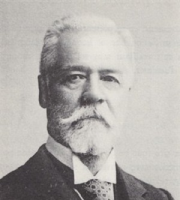
\includegraphics[scale=0.5]{Fayol}
\caption{Principal contribuyente al enfoque clásico de la administración}
\end{figure}

\item \textbf{Robert B. Buchele:} El proceso de medir los actuales resultados en relación con los planes, diagnosticando la razón de las desviaciones y tomando las medidas correctivas necesarias.
\begin{figure}[h]
\centering
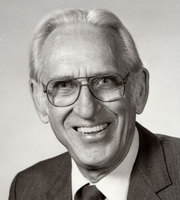
\includegraphics[scale=0.5]{Buchele}
\caption{Escritor de la Obra \textit{La gestión de empresas y organizaciones públicas}}
\end{figure}
\item \textbf{Koontz (1909-1984) \& O'Donnel (1900-1976):} Control es medir y corregir las actividades de subordinados para asegurarse que los eventos se ajustan a los planes.
\begin{figure}[h]
\centering
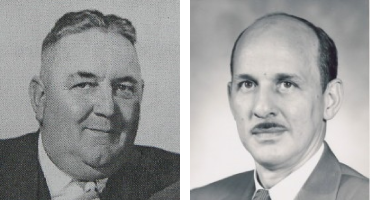
\includegraphics[scale=0.5]{KoonzODon}
\caption{Autores conjuntos de la obra \textit{Principios de Gestión} }
\end{figure}
\item \textbf{George R. Terry (1909 – 1979):} El proceso para determinar lo que se está llevando a cabo, valorización y, si es necesario, aplicando medidas correctivas, de manera que la ejecución se desarrolle de acuerdo con lo planeado.
\begin{figure}[h]
\centering
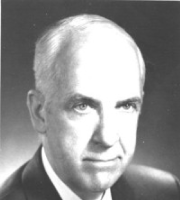
\includegraphics[scale=0.5]{Terry} 
\caption{Fue un autor de gestión estadounidense, profesor de Negocios. Se destaca por sus primeros trabajos en administración y por escribir el primer libro, titulado \textit{Principios de gestión}.}
\end{figure}
\item \textbf{Theo Haimann (1911-1989):} Control es el proceso de verificar para determinar si se están cumpliendo los planes o no, si existe un progreso hacia los objetivos
y metas. El control es necesario para corregir cualquier desviación. El
control se ejerce en todos los niveles de las organizaciones; desde
los niveles superiores o jerárquicos, hasta los niveles inferiores u
operativos.
\end{itemize}
\section{Importancia del Control}
Una de las razones más evidentes de la importancia del control es porque hasta el mejor de los planes se puede desviar. A continuación una lista de los puntos mas relevantes del control:
\begin{itemize}

\item Establece medidas para corregir las actividades, de tal forma que se alcancen planes exitosamente.
\item Se aplica a todo: a las cosas, alas personas, y a los actos.
\item Determina y analiza rápidamente las causas que pueden originar desviaciones, para que no se vuelvan a presentar en el futuro.
\item Localiza a los lectores responsables de la administración, desde el momento en que se establecen medidas correctivas.
\item Proporciona información acerca de la situación de la ejecución de los planes, sirviendo como fundamento al reiniciarse el proceso de planeación.
\item Reduce costos y ahorra tiempo al evitar errores.
\item Su aplicación incide directamente en la racionalización de la administración y consecuentemente, en el logro de la productividad de todos los recursos de la empresa.
\end{itemize}
El control cumple una función relevante en las organizaciones,en el sentido
de que las mantiene en el equilibrio deseado,tanto de ingresos, egresos, de
utilidades,de producción,de calidad de sus productos, etc. Todo sistema
requiere de equilibrio para que pueda funcionar.  \\${ }$\\
Entre otros aspectos,el control es importante para:
\begin{itemize}
\item \textbf{Crear Mejor Calidad:}  La administración de la calidad total,
conduce a grandes mejoras para el control. Las fallas del proceso se
detectan y el proceso se corrige para eliminar errores. Los empleados
tienen facultades para inspeccionar y mejorar su trabajo. La
administración de la calidad total cambia muchas de las actitudes y
los enfoques para lograr un control efectivo.
\item \textbf{Enfrentar el Cambio:}  El cambio forma parte ineludible del
ambiente de cualquier organización. Los mercados cambian,los
competidores ofrecen productos atractivos y servicios nuevos.
Surgen materiales y tecnologías más eficientes se aprueban o
enmiendan reglamentos gubernamentales. La función del control
sirve a los gerentes para responder a las amenazas o las
oportunidades de todo ello,porque les ayuda a detectarlos cambios
que están afectando los productos y servicios de sus organizaciones.
\item \textbf{Agregar Valor:}  Una ventaja competitiva en los tiempos modernos
en donde se demanda la velocidad de producción es el agregar valor
a los productos o servicios. Con frecuencia este valor agregado
adopta la forma de una calidad arriba de la media,lograda aplicando
procedimientos de control.
\item \textbf{Facilitar la Delegación y Trabajo en Equipo:} La tendencia
contemporánea hacia la administración participativa también
aumenta la necesidad de delegar autoridad y de fomentar que los
empleados trabajen juntos en equipo. Así pues,el proceso de control
permite que el gerente controle el avance de los empleados,sin
entorpecer su creatividad o participación en el trabajo.
\end{itemize}

\subsection{Areas del Control}
El control actúa en todas las áreas y en todos los niveles de la empresa. Prácticamente todas las actividades de una empresa están bajo alguna forma de control o monitoreo. Las principales áreas de control en la empresa son:
\begin{itemize}
\item \textbf{Áreas de producción:} Si la empresa es industrial, el área de producción es aquella donde se fabrican los productos; si la empresa fuera prestadora de servicios, el área de producción es aquella donde se prestan los servicios. Como ejemplo tenemos la siguiente figura:
\begin{figure}[!h]
\centering
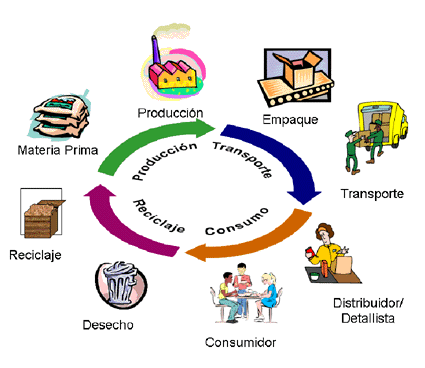
\includegraphics[scale=1.4]{CicloReciclaje}
\caption{Grafica que Ilustra el Ciclo de Venta de Cajas de Cartón}
\end{figure}
\item \textbf{Control de producción:} El objetivo fundamental de este control es programar, coordinar e implantar todas las medidas tendientes a lograr un optima rendimiento en las unidades producidas, e indicar el modo, tiempo y lugar más idóneos para lograr las metas de producción, cumpliendo así con todas las necesidades del departamento de ventas. 
\end{itemize}
\section{Principios}
La aplicación racional del control debe fundamentarse en los siguientes principios:
\begin{itemize}
\item \textbf{Equilibrio:} A cada grupo conferido debe proporcionarse al grado del control correspondiente. De la misma manera que la autoridad se delega y la responsabilidad se comparte, al delegar autoridad es necesario establecer los mecanismos suficientes para verificar que se esta cumpliendo con la responsabilidad conferida, y que la autoridad delegada esta siendo debidamente ejercida.
\item \textbf{De los Objetivos:} Se refiere a que el control existe en función de los objetivos, es decir, el control no es un fin, sino un medio para alcanzar los objetivos preestablecidos.
\item \textbf{De la Oportunidad:} El control, para que sea eficaz, necesita ser oportuno, es decir, debe aplicarse antes de que se efectúe el error. De tal manera que sea posible tomar medidas correctivas, con anticipación.
\item \textbf{De las Desviaciones:} Todas las variaciones o desviaciones que se presenten en relación con los planes deben ser analizadas detalladamente, de tal manera que sea posible conocer las causas que las originaron, a fin de tomar las medidas necesarias para evitarlas en el futuro.
\item \textbf{Costeabilidad: }Es establecimiento de un sistema de control debe justificar el costo que este represente en tiempo y dinero, en relaciona con las ventajas reales que este reporte.
\item \textbf{Excepción:} El control debe aplicarse, preferentemente, a las actividades excepcionales o representativas, a fin de reducir costos y tiempo, delimitando adecuadamente cuales funciones estratégicas requiere el control.
\item \textbf{De la Función Controlada:} La función controlada por ningún motivo debe comprender a la función controlada, ya que pierde efectividad el control. Este principio es básico, ya que señala que la persona o la función que realiza el control no debe estar involucrada con la actividad a controlar.

\end{itemize}

\section{Reglas del Control}
\begin{enumerate}
\item	\textit{Establecimiento de los medios de control.}
\item	\textit{Operaciones de recolección de datos.}
\item	\textit{Interpretación y valoración de los resultados.}
\item	\textit{Utilización de los mismos resultados.}
\end{enumerate}
La primera,y la última de estas etapas son esencialmente propias del
administrador.
La segunda,ciertamente es del técnico en el control de que se trate. La
tercera,suele ser del administrador,con la ayuda del técnico.
\subsection{Procesos del Control}
El control es un proceso cíclico y repetitivo. Está compuesto de cuatro elementos que se suceden:
\begin{itemize}
\item \textbf{Establecimiento de estándares:} Es la primera etapa del control, que establece los estándares o criterios de evaluación o comparación. Un estándar es una norma o un criterio que sirve de base para la evaluación o comparación de alguna cosa. Existen cuatro tipos de estándares; los cuales se presentan a continuación:
\begin{itemize}
\item \textit{Estándares de cantidad:} Como volumen de producción, cantidad de existencias, cantidad de materiales primas, números de horas, entre otros.
\item \textit{Estándares de calidad:} Como control de materia prima recibida, control de calidad de producción, especificaciones del producto, entre otros.
\item \textit{Estándares de tiempo:} Como tiempo estándar para producir un determinado producto, tiempo medio de existencias de un productos determinado, entre otros.
\item \textit{Estándares de costos:} Como costos de producción, costos de administración, costos de ventas, entre otros.
\end{itemize}
\end{itemize}

\begin{figure}[h]
\begin{adjustbox}{width=\textwidth}
\begin{tabular}{|c|c|c|c|}

\hline 
Estandares & \thead{Fabrica de \\ Alfajores} & \thead{Empresa\\ Lechera} & Agencia de Viajes \\ 
\hline 
Cantidad & Volumen de Alfajores & Litros de Leche & Pasajeros/Vuelos \\ 
\hline 
Calidad & Sabor/Frescura & Cuerpo(tenor,graso) & Categorias \\ 
\hline 
Tiempo & \thead{Producción Diaria\\Mensual\\Venta Diaria\\Mensual}  & Produccion Diaria/Mensual & \thead{Tiempo de Vuelo\\Duracion del Tour} \\ 
\hline 
Costo & Costo del Alfajor & Relacion Leche/Crema & Costo del Tour \\ 
\hline 
\end{tabular} 
\end{adjustbox}
\caption{Tabla de ejemplo para los tipos de Estándares en tres Empresas Hipoteticas Distintas}
\end{figure}

\begin{itemize}
\item \textbf{Evaluación del desempeño:} Es la segunda etapa del control, que tiene como fin evaluar lo que se está haciendo.
\item \textbf{Comparación del desempeño con el estándar establecido:} Es la tercera etapa del control, que compara el desempeño con lo que fue establecido como estándar, para verificar si hay desvío o variación, esto es, algún error o falla con relación al desempeño esperado.
\item \textbf{Acción correctiva:} Es la cuarta y última etapa del control que busca corregir el desempeño para adecuarlo al estándar esperado. La acción correctiva es siempre una medida de corrección y adecuación de algún desvío o variación con relación al estándar esperado.
\end{itemize}
Los controles deben ser flexibles. Cuando un control no es flexible,un
problema que exija rebasarlo calculado en la previsión,hace que,o bien no
pueda adecuadamente la función,o bien se tienda a abandonar el control
como inservible. Muchos están en contra del empleo de controles,
precisamente por su inflexibilidad.



\begin{figure}[ht]
\centering
\begin{tikzpicture}
\matrix [column sep=7mm, row sep=5mm] {
  \node (se) [draw, shape=rectangle] {Establecimiento de Estandares}; &
  \node (ul) [draw, shape=rectangle] {Evaluación de Desempeño}; \\
  \node (we) [draw, shape=rectangle] {Evaluación de  Resultados}; &
  \node (pu) [draw, shape=rectangle] {Retroalimentación (Acción Correctiva)}; \\
};
\draw[thick,-Latex] (se) -- (ul);
\draw[thick,-Latex] (ul) -- (pu);
\draw[thick,-Latex] (pu) -- (we);
\draw[thick,-Latex] (we) -- (se);

\end{tikzpicture}
\caption{Gráfica que representa los Procesos del Control}
\end{figure}
\subsection{Finalidad}
\begin{itemize}
\item \textbf{Informar:} es necesario transmitir y comunicar la información para la toma de decisiones e identificar los factores claves de la organización.
\item \textbf{Coordinar:} Encamina las actividades a realizar eficazmente a la obtención de los objetivos.
\item \textbf{Evaluar:} La consecución de las metas u objetivos se logra gracias a las personas y su valoración es la que pone de manifiesto la satisfacción del logro.
\item \textbf{Motivar:} El impulso y la ayuda es de mucha importancia para alcanzar las metas.
\end{itemize}

\section{Conclusión}
El control es una función administrativa: es la fase del proceso administrativo que mide y evalúa el desempeño y toma la acción correctiva cuando se necesita. De este modo, el control es un proceso esencialmente regulador. \\${ }$\\
Para que el control sea efectivo debe desarrollarse como una unidad y aplicarse en todo tiempo a la empresa, pudiendo clasificarse en: 
\begin{itemize}
\item Control Preliminar
\item Control Concurrente 
\item Control Posterior
\end{itemize}
La aplicación de un control en las organizaciones busca atender dos finalidades principales: Corregir fallas o errores existentes y Prevenir nuevas fallas o errores de los procesos. 

\newpage


\begin{thebibliography}{9}
\bibitem{Tecnologico} 
Elvina Solano.
\textit{Control como Funcion Administrativa}. 
Tecnologico de Estudios Superiores de Chimalhuacán, 2013.
 
\bibitem{Rafael} 
Rafael Franco Ruíz. \textit{Revista Nº 5 - Evolución histórica del control}, legal.legis.com.co, 2001.

 
\bibitem{Monografias} 
Marco Antonio. \textit{Concepto, Importancia y Principios del Control}, monografias.com, 2010.
\\\texttt{http://www.monografias.com/trabajos11/prico/prico.shtml}

\bibitem{Altamira} 
Laura Esmeralda. \textit{Antecedentes del Control  Administrativo}, Instituto Tecnológico de Altamira., 2010.

\bibitem{Adm1}
Walter Parada Ruiz. \textit{Administración I, Compilación Bibliografica}, Facultad de Ciencias Economicas y Financieras, Universidad Autónoma Gabriél Rene Moreno.

\bibitem{Edd}
Eddy Escalate Ustariz, Robert Gutierrez Rodriguez, Marco Antonio Mamani Iquise. \textit{Informe: El Control}, Universidad Autonoma Gabriel Rene Moreno, 2012.

\bibitem{yuri}
Elibeth Yuri. \textit{El Control}, monografias.com, 2010.
\\\texttt{https://www.monografias.com/trabajos14/control/control.shtml}
\end{thebibliography}



\end{document}
